To evaluate the structural validity and predictive reliability of the developed Agent-Based Model (ABM), a Global Sensitivity Analysis (GSA) using Sobol indices was executed. Unlike local sensitivity analysis, GSA accounted for the non-linear interactions between variables across the entire multi-dimensional input space \citep{Sobol2001}. This stress-testing phase involved varying the five core behavioral parameters ($w_a, w_{sn}, w_{pbc}, c_{\text{effort}}, \text{decay}$) by $\pm 20\%$ to quantify their individual contributions ($S_1$) to the variance in global compliance rates.

\begin{figure}[htbp]
    \centering
    % Ensure the filename matches exactly (case-sensitive on Overleaf/Linux)
    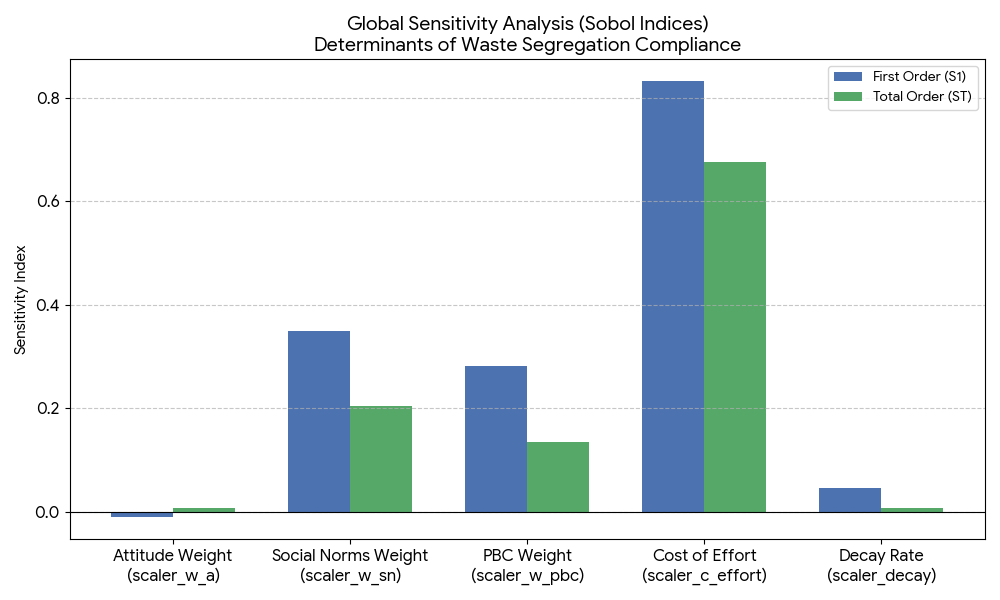
\includegraphics[width=0.8\textwidth]{Sobol.png}
    \caption{Global Sensitivity Analysis Results illustrating First-Order Sobol Indices ($S_1$) for behavioral parameters.}
    \label{fig:sobol_analysis}
\end{figure}